%--------------------
% Packages
% -------------------
\documentclass[11pt,a4paper]{article}
\usepackage[utf8x]{inputenc}
%\usepackage{gentium}

\usepackage[pdftex]{graphicx} % Required for including pictures
\usepackage[pdftex,linkcolor=black,pdfborder={0 0 0}]{hyperref} % Format links for pdf
\usepackage{calc} % To reset the counter in the document after title page
\usepackage[english]{babel}     % for proper word breaking at line ends
\usepackage{graphicx}           % for ?
\usepackage{amsmath,amssymb}    % for better equations
\usepackage{amsthm}             % for better theorem styles
\usepackage{mathtools}          % for greek math symbol formatting
\usepackage{varwidth}
\usepackage{enumitem}           % for control of 'enumerate' numbering
\usepackage{listings}           % for control of 'itemize' spacing
 \setlength {\marginparwidth }{2cm}
\usepackage{todonotes}          % for clear TODO notes
\usepackage{pgfplots}
\usepackage{caption}
\usepackage{parskip}
\usepackage{makecell}
\usepackage{tabularx} 

\usepackage[a4paper, lmargin=0.1666\paperwidth, rmargin=0.1666\paperwidth, tmargin=0.1111\paperheight, bmargin=0.1111\paperheight]{geometry} %margins
%\usepackage{parskip}

\usepackage[all]{nowidow} % Tries to remove widows
\usepackage[protrusion=true,expansion=true,stretch=10]{microtype} % Improves typography, load after fontpackage is selected
\usepackage{hyperref}

\title{Research proposal master thesis: \\ Authenticated video calls in PubHubs}
\author{Julian van der Horst}

%-----------------------
% Begin document
%-----------------------
\begin{document} 
\maketitle
\section{Introduction}
This document will outline the research I will be doing for my master thesis.

In general, we will do research into authenticated video calling in PubHubs. The research will be about the challenges and architectural designs needed to make such a feature, particularly looking into the security and privacy aspects of such a system and keeping them in line with the security and privacy considerations already made in PubHubs. We will propose and build a video calling solution and discuss the compromises, limitations and dependencies. 

This research will also include a section on discussing the current landscape of authenticated video calls. We will consider other alternatives and look at the importance of authenticated video calls following recent events.

\section{PubHubs}
Let us start by introducing PubHubs. PubHubs, short for Public Hubs, is an alternative community platform that puts public values first \cite{PH}. Unlike mainstream social media platforms like Instagram or Twitter that focus on individual broadcasting, PubHubs emulates real-world social dynamics by centering interactions within smaller, community-based hubs. The reasoning behind that is that this behavior closely resembles normal human interaction, where humans have small groups of friends with whom they interact. The way people experience social media now is very unnatural, where if they engage with a platform it is shouted into the whole world.

"PubHubs is organized as a network of independent hubs, with a shared single-sign-on. Conversations take place in local hubs (and not globally) and the associated (conversation) data is managed decentrally, within each hub" \cite{PH}. Privacy is one of the core values of PubHubs, which can be seen in how it handles identity management. The main idea of Pubhubs is to allow anonymity but still have accountability and still have the ability to verify certain attributes of the user. The authentication of users is done using Yivi (formerly IRMA)\cite{YIVI} and the identity (the pseudonym) is generated using PEP \cite{PEP}.

\section{Video conferencing}
During the COVID-19 pandemic, there was a big need for remote work. Immediately, services like Zoom \cite{Zoom}  and Microsoft Teams  \cite{MSTeams} gained widespread adoption. These tools allowed video conferencing between different remote locations in real-time. These video call services might include end-to-end encryption but often lack authenticated video calls. Perhaps the need for authenticated video calls is not very apparent, and when calling friends it might not be needed. On the contrary, when having an online consultation with your doctor, you want to be sure that you are actually calling a doctor.

If we look at video conferencing from a conceptual perspective, we see that there are multiple conferencing setups. For this research, we will distinguish three types. Person-to-person (one-on-one), Person-to-person (multiple people), and speaker-to-audience. We distinguish these types because they all have certain properties that make it so that different technologies are a better fit for that type. Where in one-on-one we only need to send and receive to one other person, when we are in a group we need to send and receive data to each member in a call. On the contrary with speaker-to-audience, we do not have connections between the individual audience members. In this research we will mostly focus on the first and second setup.

\begin{figure}[!hbt]
    \centering
    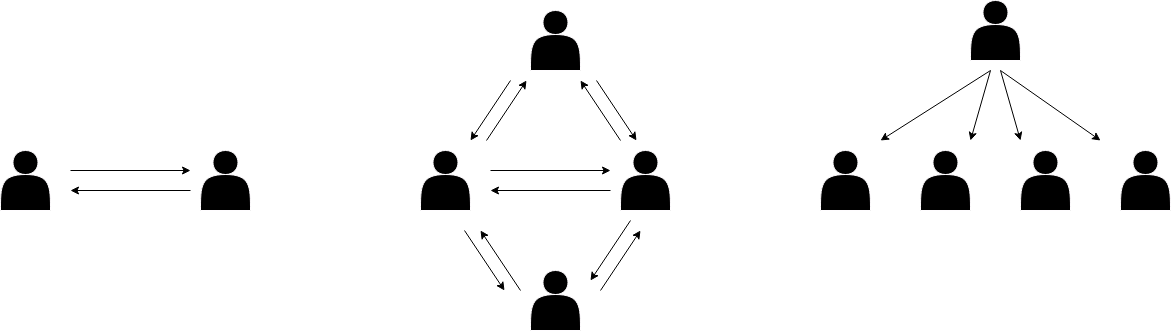
\includegraphics[width=0.7\textwidth]{Research proposal/img/three types.drawio.png}
    \caption{The three types of video calling}
    \label{fig:enter-label}
\end{figure}

With video conferencing, people need to send and receive video streams, and we want to do this ideally in real time. A standard for that is WebRTC, and it is now widely supported in browsers (97.77\%) \cite{CIUIWEBRTC}. WebRTC is both a protocol and an API that can be used for many things including video and audio communication. Matrix even has support for WebRTC and uses it in their main testing application Element \cite{ELEMENT}. We will use WebRTC in our implementation to send the video and audio streams, however to what do we need to send these WebRTC streams?

We either send the data in a P2P network. This means that the people in the call send their stream to every other person in the call. This makes it so that the server has no extra load since it does not handle any video streams in only initially facilitates the call setup. However, with every extra participant, every user needs to send/receive more and more data. At some point a bottleneck is reached, and no extra participant can be added or a loss in data will occur. This is a very privacy-friendly method since the server has no access to the video call data being sent.

Another option would be to have an MCU. An MCU takes in many media streams and combines them into one media stream. This makes it so that it can work very well with legacy systems, since an MCU can receive various types of media and then output a standardized output. For example, this would allow a participant calling in from a phone connection while the other participant have a video call. The MCU has to decode all the incoming media signals, which makes it costly at large scale, since the CPU usage would be very high. From a security and privacy perspective this solution is not ideal, since the server has access to all the unencrypted video and audio data.

Lastly, we have the SFU. An SFU behaves in a way like a switch where it would selectively forward streams between clients, it does not interact with the video streams so it would work similarly with encrypted and unencrypted data. For a user perspective, we only need to talk to one server, and we send and receive all our data through that server. An SFU provides a compelling balance of scalability and privacy. it needs lower resources since it only needs to forward the signals to the users and does not decrypt the data. 

\section{Matrix and Element call}
In PubHubs all communication is done via Matrix. "Matrix is an open source network for secure, decentralized communication" \cite{MATRIX}. The community can suggest changes to the Matrix protocol by submitting proposals, over the years this has added a lot of functionality to Matrix. In proposal 3401 \cite{MATRIX_VIDEO_CALL_PROP}, functionality for video calling was proposed. This proposal can be applied to all the above-mentioned server setups and describes a protocol for video calling. 

The same team that built matrix is also building Element \cite{ELEMENT}, which is an open-source implementation of a messaging app that uses matrix. A new feature was added to Element called Element call, which serves as an example implementation of the proposal mentioned above. They started by using peer-to-peer video calling since this more closely resembled the decentralized infrastructure of Matrix. However, this turned out to not be the best solution since it allowed for a maximum of 7 participants and video calling required lots of computer resources from participants. Recently they have released a new version that makes use of an open-source SFU called Livekit \cite{LIVEKIT}.

We will use this implementation as a guide during our research, however, we will evaluate all the different choices made for Element call and deviate from them based on the requirements of PubHubs. When using Livekit we can very easily implement features like noise suppression or video simulcast (Sending multiple video stream with different qualities, to dynamically choose the quality according to your internet connection).

\section{Research question}
The main research question will be \"How can we design and implement an authenticated video calling solution within PubHubs that balances privacy, security, and usability?\". This question then raises several sub-questions, questions like: What information should we allow leaking with regard to the current Pubhubs privacy framework?. Should we allow users to see that other users are on a call? Should we allow users to call peer-to-peer and thus have no moderation? How to do encrypted video calls in PubHubs? Encryption can be done in multiple ways, do we want our users to have to share keys, or can this be done using PEP or Yivi?

While doing the research and writing the code for it, we should also keep in mind the current development setup for PubHubs. This means that we should keep in mind which technologies they are using now and remain in those ecosystems. This makes it so that the code can be more easily maintained in the future. Learning this environment and adapting the code to their existing setup can be quite a challenge.

As mentioned previously, we will also discuss authenticated video calls from a bigger perspective and discuss questions like: why has authenticated call not taken of? How do important institutions, like hospitals, do this now? Especially now, with generating AI videos becoming a trivial task, the need for authenticated video calls will be higher. 

\bibliographystyle{plain}
\bibliography{main.bib}

\end{document}
